%% 
%% Copyright 2007-2020 Elsevier Ltd
%% 
%% This file is part of the 'Elsarticle Bundle'.
%% ---------------------------------------------
%% 
%% It may be distributed under the conditions of the LaTeX Project Public
%% License, either version 1.2 of this license or (at your option) any
%% later version.  The latest version of this license is in
%%    http://www.latex-project.org/lppl.txt
%% and version 1.2 or later is part of all distributions of LaTeX
%% version 1999/12/01 or later.
%% 
%% The list of all files belonging to the 'Elsarticle Bundle' is
%% given in the file `manifest.txt'.
%% 
%% Template article for Elsevier's document class `elsarticle'
%% with harvard style bibliographic references

\documentclass[preprint,12pt,authoryear]{elsarticle}

%% Use the option review to obtain double line spacing
%% \documentclass[authoryear,preprint,review,12pt]{elsarticle}

%% Use the options 1p,twocolumn; 3p; 3p,twocolumn; 5p; or 5p,twocolumn
%% for a journal layout:
%% \documentclass[final,1p,times,authoryear]{elsarticle}
%% \documentclass[final,1p,times,twocolumn,authoryear]{elsarticle}
%% \documentclass[final,3p,times,authoryear]{elsarticle}
%% \documentclass[final,3p,times,twocolumn,authoryear]{elsarticle}
%% \documentclass[final,5p,times,authoryear]{elsarticle}
%% \documentclass[final,5p,times,twocolumn,authoryear]{elsarticle}

%% For including figures, graphicx.sty has been loaded in
%% elsarticle.cls. If you prefer to use the old commands
%% please give \usepackage{epsfig}

%% The amssymb package provides various useful mathematical symbols
\usepackage{amssymb}
%% The amsthm package provides extended theorem environments
%% \usepackage{amsthm}

%% The lineno packages adds line numbers. Start line numbering with
%% \begin{linenumbers}, end it with \end{linenumbers}. Or switch it on
%% for the whole article with \linenumbers.
%% \usepackage{lineno}

\journal{Ocean Engineering}

\begin{document}

\begin{frontmatter}

    %% Title, authors and addresses

    %% use the tnoteref command within \title for footnotes;
    %% use the tnotetext command for theassociated footnote;
    %% use the fnref command within \author or \affiliation for footnotes;
    %% use the fntext command for theassociated footnote;
    %% use the corref command within \author for corresponding author footnotes;
    %% use the cortext command for theassociated footnote;
    %% use the ead command for the email address,
    %% and the form \ead[url] for the home page:
    %% \title{Title\tnoteref{label1}}
    %% \tnotetext[label1]{}
    %% \author{Name\corref{cor1}\fnref{label2}}
    %% \ead{email address}
    %% \ead[url]{home page}
    %% \fntext[label2]{}
    %% \cortext[cor1]{}
    %% \affiliation{organization={},
    %%            addressline={}, 
    %%            city={},
    %%            postcode={}, 
    %%            state={},
    %%            country={}}
    %% \fntext[label3]{}

    \title{Adopting a laboratory system based manoeuvring model to a real sea environment}

    %% use optional labels to link authors explicitly to addresses:
    %% \author[label1,label2]{}
    %% \affiliation[label1]{organization={},
    %%             addressline={},
    %%             city={},
    %%             postcode={},
    %%             state={},
    %%             country={}}
    %%
    %% \affiliation[label2]{organization={},
    %%             addressline={},
    %%             city={},
    %%             postcode={},
    %%             state={},
    %%             country={}}

    \author[1,3]{Martin Alexandersson\corref{cor1}%
        %\fnref{fn1,fn3}
    }
    \ead{maralex@chalmers.se}

    \author[2]{Ulysse Dhomé}
    \author[3]{Wengang Mao}
    \author[4]{Jonas W. Ringsberg}


    \affiliation[1]{organization={Dept. of Mechanics and Maritime Sciences, Division of Marine Technology, Chalmers University of Technology},%Department and Organization
        addressline={Hörsalsvägen 7A},
        city={Gothenburg},
        postcode={41296},
        country={Sweden}}

    \affiliation[2]{organization={KTH Royal Institute of Technology},%Department and Organization
        %addressline={Hörsalsvägen 7A},
        %city={Gothenburg},
        %postcode={41296},
        country={Sweden}}

    \affiliation[3]{organization={Research Institutes of Sweden (RISE)},%Department and Organization
        addressline={Chalmers tvärgata 10},
        city={Gothenburg},
        postcode={41296},
        country={Sweden}}

    \cortext[cor1]{Corresponding author}

    \begin{abstract}
        %% Text of abstract

    \end{abstract}

    %%Graphical abstract
    %\begin{graphicalabstract}
    %    %\includegraphics{grabs}
    %\end{graphicalabstract}
    %
    %%%Research highlights
    %\begin{highlights}
    %    \item Research highlight 1
    %    \item Research highlight 2
    %\end{highlights}

    \begin{keyword}
        %% keywords here, in the form: keyword \sep keyword

        %% PACS codes here, in the form: \PACS code \sep code

        %% MSC codes here, in the form: \MSC code \sep code
        %% or \MSC[2008] code \sep code (2000 is the default)

    \end{keyword}

\end{frontmatter}

%% \linenumbers

%% main text
%\section{}
%\label{}
\section{Introduction}
\label{sec:introduction}
\section{Method}
\label{sec:method}
\input{datasets.tex}
\subsection{Ship scale models}
\label{sec:ship_scale_models}
The data was collected with two scale models of the wPCC. The smaller 5m model (see \autoref{fig:5m}) with scale factor 1:41 was used in the laboratory experiments. The larger 7m geosim model (see \autoref{fig:7m}) with scale factor 1:30 was used in the field data experiments. The main particulars of the two models are shown in \autoref{tab:main_particulars}. The two models are almost geometrically similar; the only exceptions are: that the rudders of the 7m models are slightly more to the aft (5 cm), the 5m model has two stabilizer fins (see \autoref{fig:5m}), and that the propeller geometries are different. The geometries differ above the water line however, where the 7m model has a large positive bow angle.
\begin{table}[!ht]
    \centering
    \caption{Main particulars of the 5m and 7m scale models.}
    \label{tab:main_particulars}
    \pgfplotstabletypeset[col sep=comma,
        columns={Particular,Unit,5m,7m},
        columns/Particular/.style={string type},
        columns/Unit/.style={string type},
        columns/5m/.style={string type},
        columns/7m/.style={string type},
        column type=l,	% specify the align method
        every head row/.style={before row=\hline,after row=\hline},	% style the first row
        every last row/.style={after row=\hline},	% style the last row
    ]{tables/ship_main_particulars.main_particulars.csv"}
\end{table}
\begin{figure}[!ht]
    \includegraphics[width=\textwidth]{figures/5m.jpg}
    \caption{5m model. One of the stabilizer fins can be seen at the bilge around the midship section. It can also be seen that the model was equiped with two fans, to test the sailing performance of the ship. These fans are however not used in this paper.}
    \label{fig:5m}
\end{figure}
\begin{figure}[!ht]
    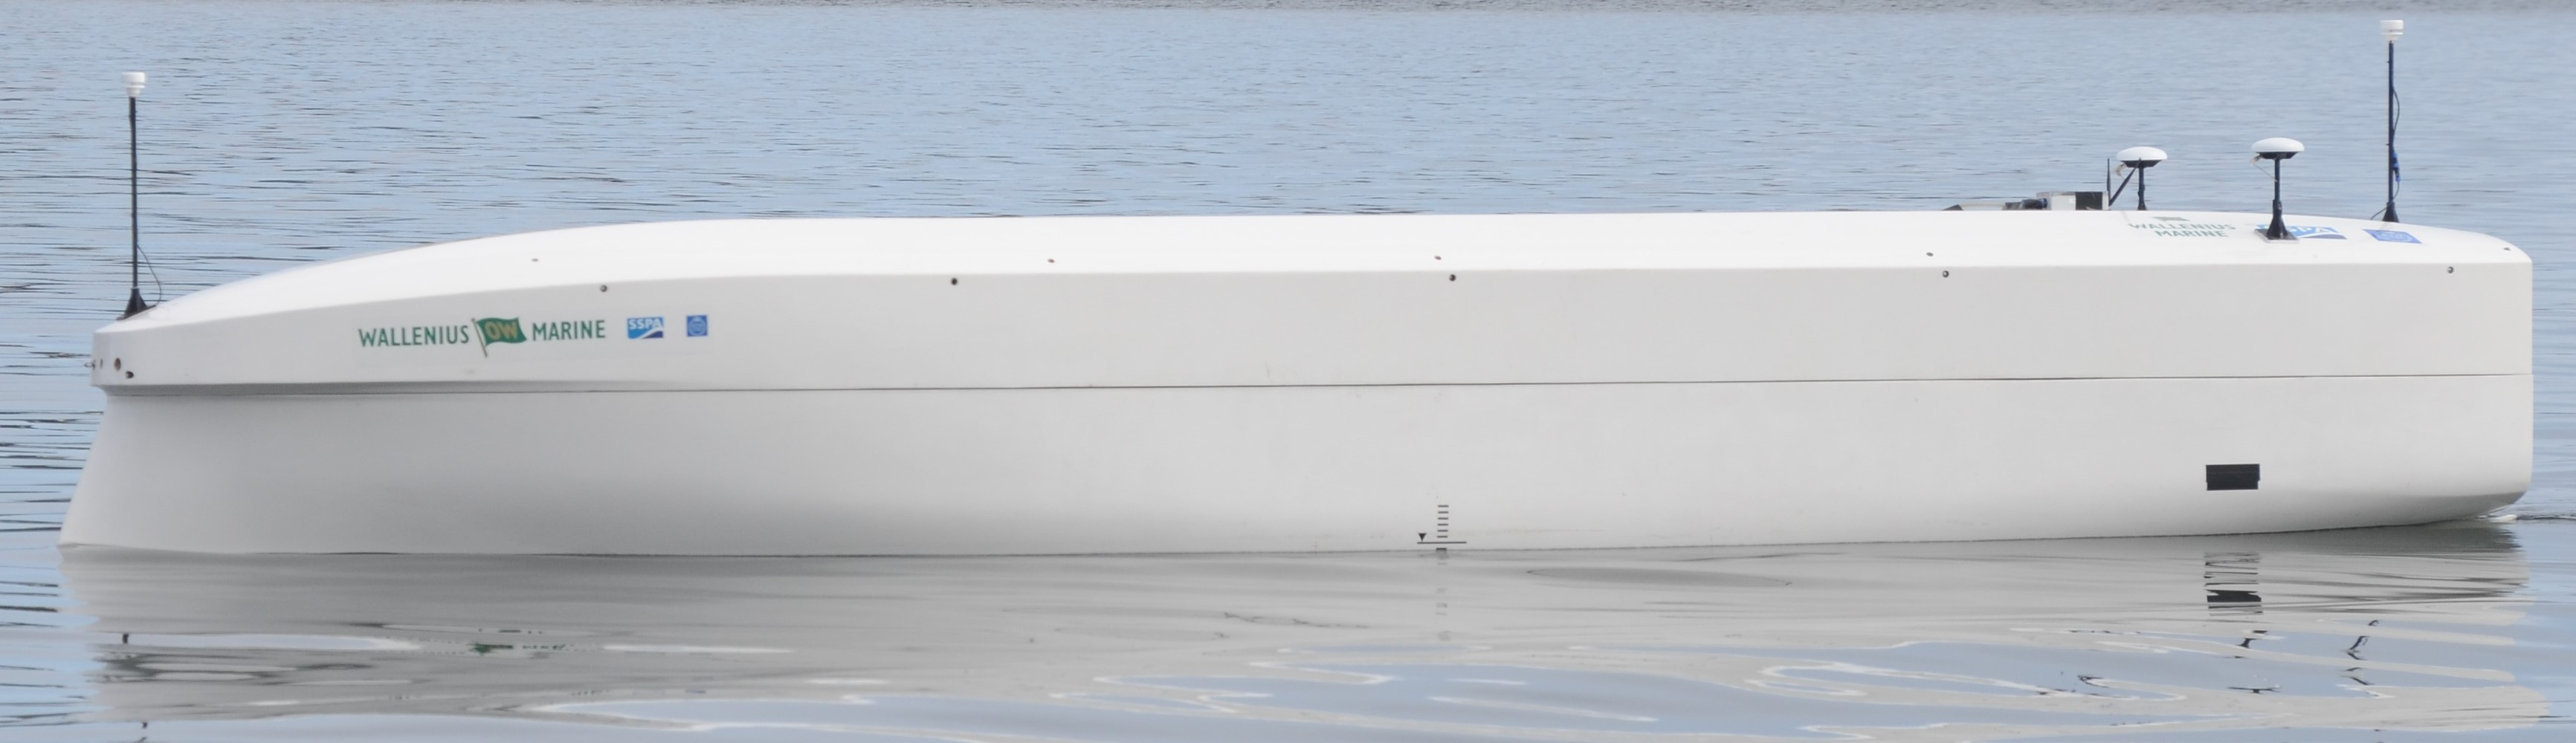
\includegraphics[width=\textwidth]{figures/7m.jpg}
    \caption{7m model. The bow and aft anemometers and the two GPS antennas, in the aft, can be seen ontop of the superstructure.}
    \label{fig:7m}
\end{figure}
\subsection{Scaling}
\label{sec:scale_effects}
Scaling procedures need to be applied in order to relate the results from the smaller 5m model to the larger 7m model. The prime system and Froude scaling are used in this paper. The prime system can be used to express the results and ship main particulars in nondimesional units. This system can be used to relate the forces and moments and to create nondimesional mathematical models that can be used for both the 5m and 7m models. The Froude scaling is applied for surface ships \citep{ittc_ittc_2008} to scale the 5m results to 7m scale in SI units. The Froude scaling between the 5m and 7m models is shown in \autoref{eq:froude_scaling}.
\begin{equation}
    \label{eq:froude_scaling}
    \begin{split}
        L_{7m} = L_{5m} \cdot \lambda \\
        V_{7m} = V_{5m} \cdot \sqrt{\lambda}
    \end{split}
\end{equation}
The scale factor $\lambda=1.373$ in this case, since the 7m is that much longer. The prime system and Froude scaling are summarized in \autoref{tab:scalings} where the prime system column contains the multiplication factor from prime system to SI units. The Froude scaling column contains the multiplication factor from model scale to full scale.

\begin{table}[!ht]
    \centering
    \caption{Scalings with prime system and Froude scaling.}
    \label{tab:scalings}
    \pgfplotstabletypeset[col sep=comma,
        columns={Physical quantity,SI unit,Prime system,Froude scaling},
        columns/SI unit/.style={string type},
        columns/Physical quantity/.style={string type},
        columns/Prime system/.style={string type},
        columns/Froude scaling/.style={string type},
        column type=l,	% specify the align method
        every head row/.style={before row=\hline,after row=\hline},	% style the first row
        every last row/.style={after row=\hline},	% style the last row
    ]{tables/scale_effects.scalings.csv"}
\end{table}



\section{Results}
\label{sec:results}
\input{froude_scaling.tex}
\section{Conclusions}
\label{sec:conclusions}

%% The Appendices part is started with the command \appendix;
%% appendix sections are then done as normal sections
%% \appendix

%% \section{}
%% \label{}

%% If you have bibdatabase file and want bibtex to generate the
%% bibitems, please use
%%
%%  \bibliographystyle{elsarticle-harv} 
%%  \bibliography{<your bibdatabase>}

%% else use the following coding to input the bibitems directly in the
%% TeX file.

\begin{thebibliography}{00}

    %% \bibitem[Author(year)]{label}
    %% Text of bibliographic item

    \bibitem[ ()]{}

\end{thebibliography}
\end{document}

\endinput
%%
%% End of file `elsarticle-template-harv.tex'.
